\documentclass[report]{nrel}

\usepackage{import}
\usepackage{longtable}

\begin{document}
\tableofcontents

\chapter{Stations in this area}

\input{StationsTable}

% map of stations
\begin{figure}[!ht]
\centering
\includegraphics[width = 6in]{../maps/MapOfStationsByID}
\caption{Station locations.}
\end{figure}

\section{Data Availability}

\begin{figure}[!ht]
\centering
\includegraphics[width = 6in]{../figures/PlotOfDataCountByYear}
\caption{Data availability. Plots show the number of valid data points per station by measured value, per year.}
\end{figure}

\chapter{Regional wind speeds}
\section{Maps}

% mean wind speeds
\begin{figure}[!ht]
\centering
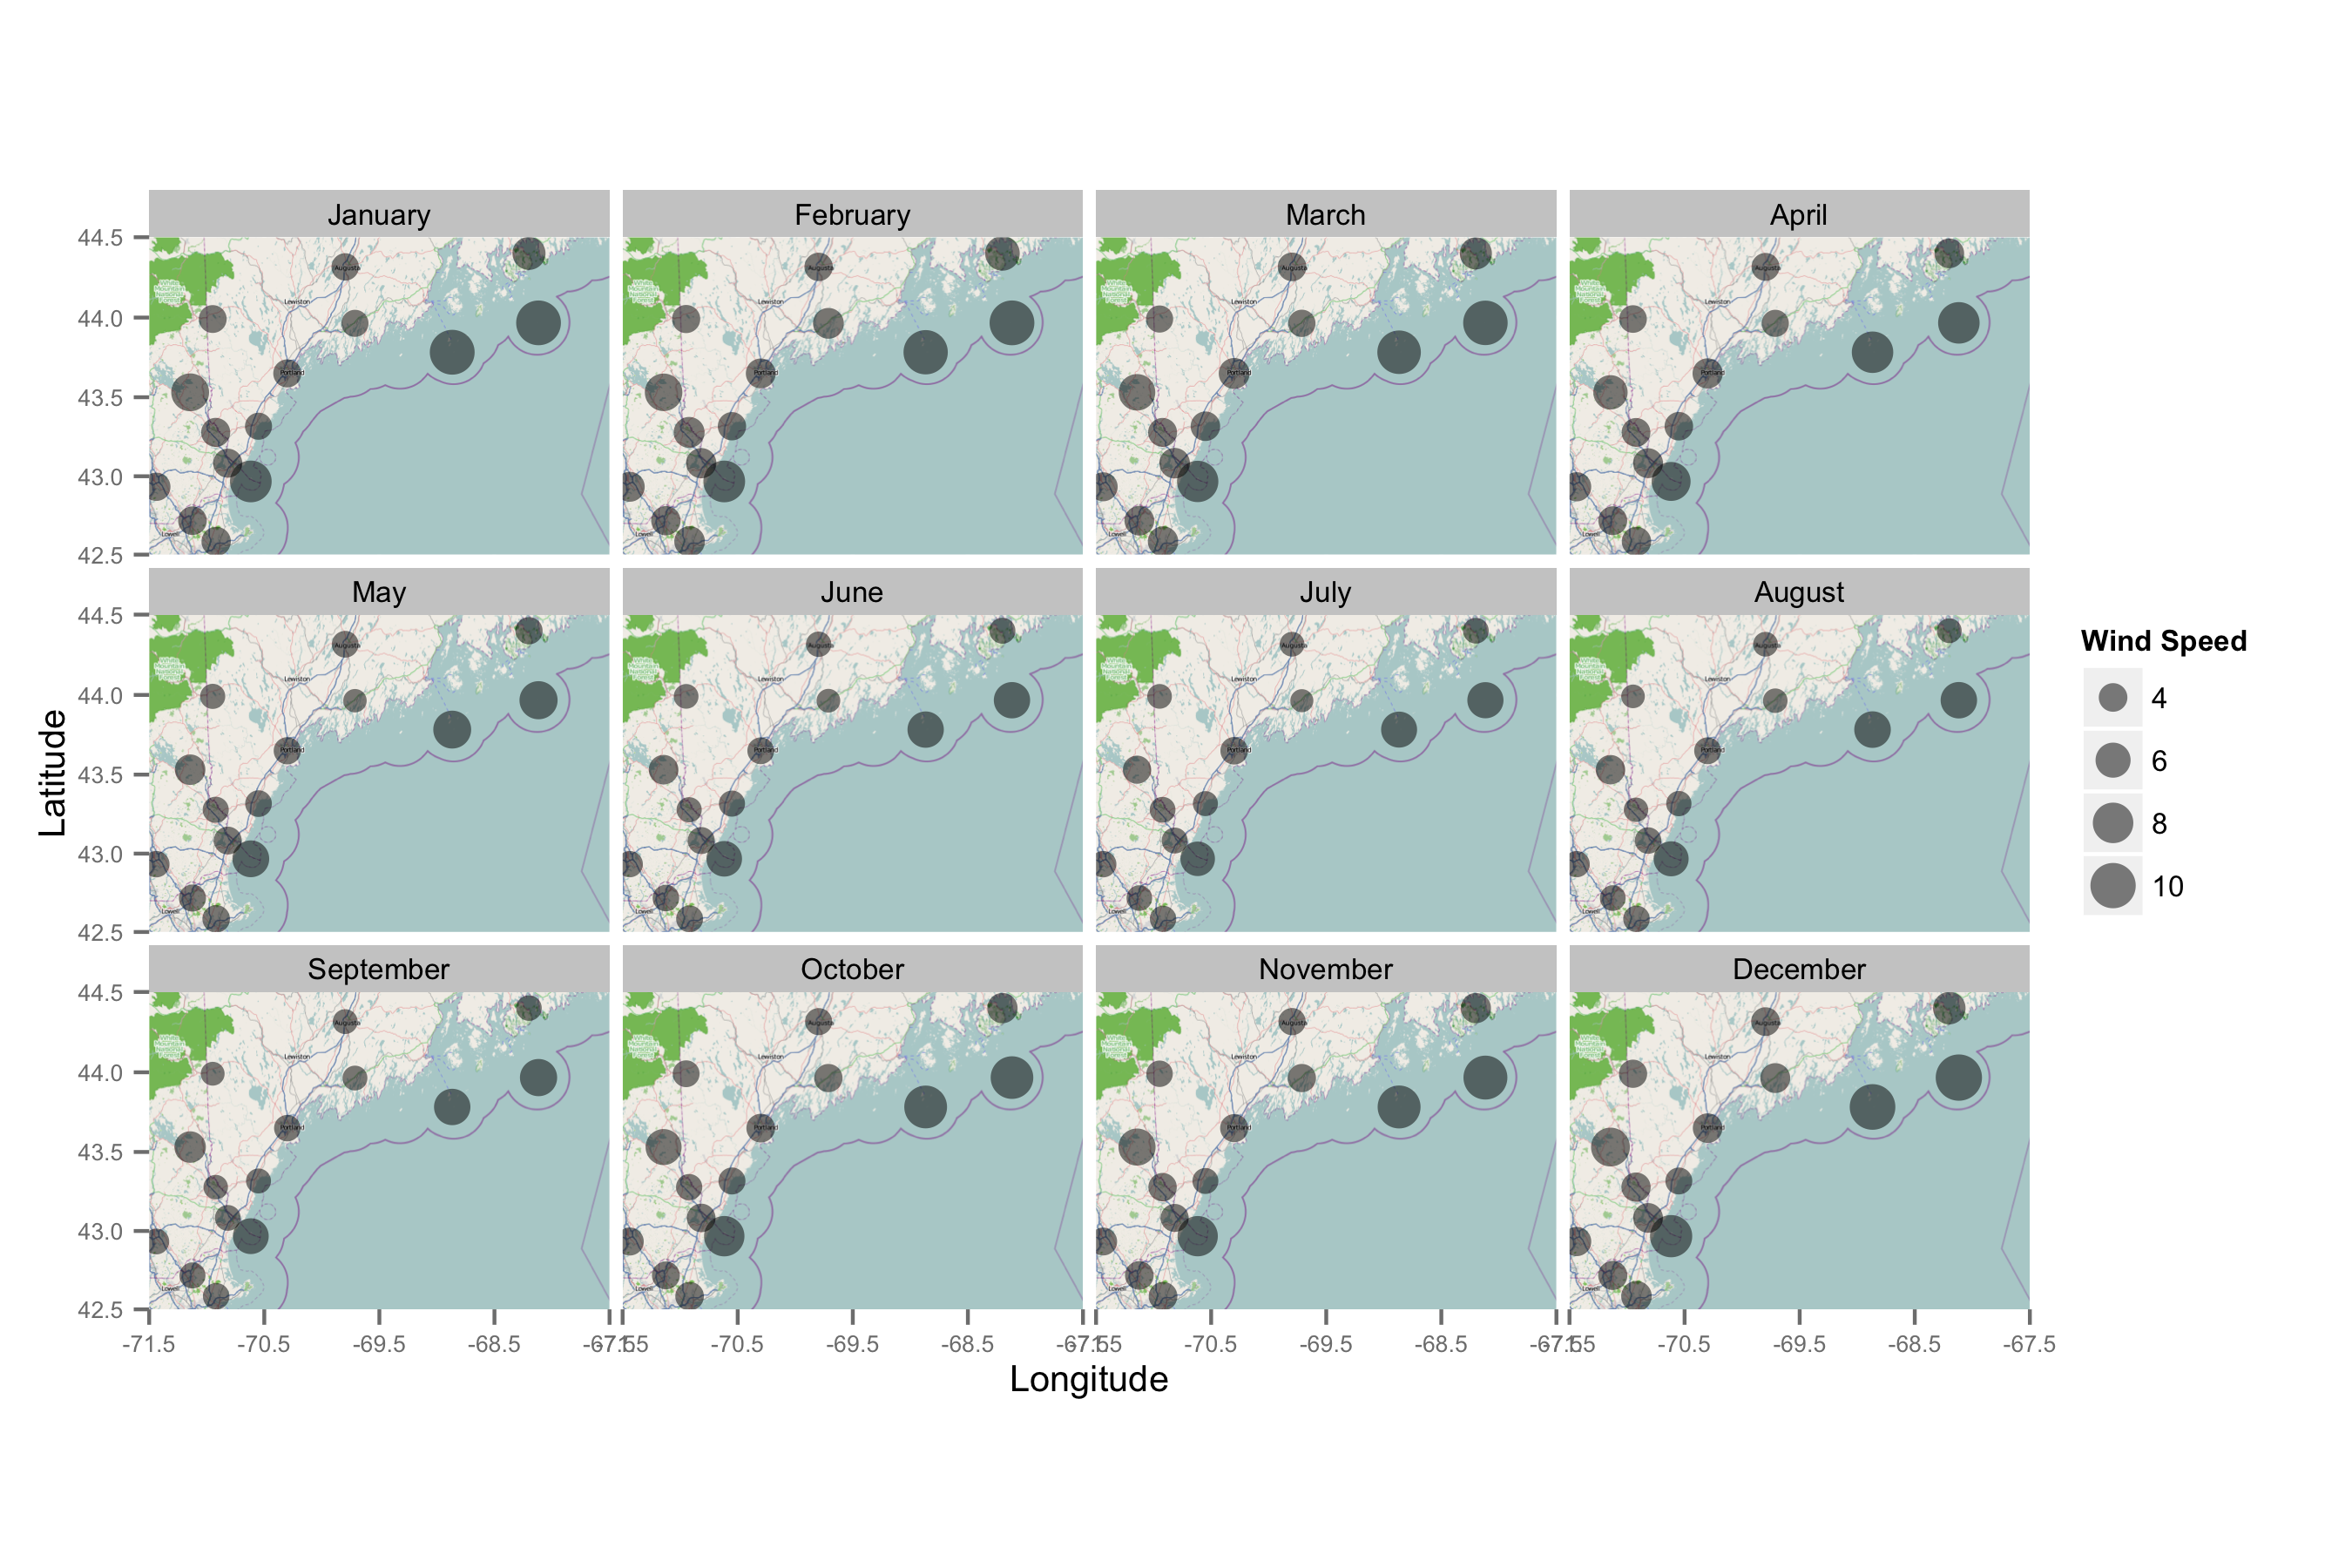
\includegraphics[width = 6in]{../maps/MapMonthlyMeanWindSpeed}
\caption{Mean wind speeds. Marker colors show the monthly means of all of the daily mean wind speeds.}
\end{figure}

% maximum wind speeds
\begin{figure}[!ht]
\centering
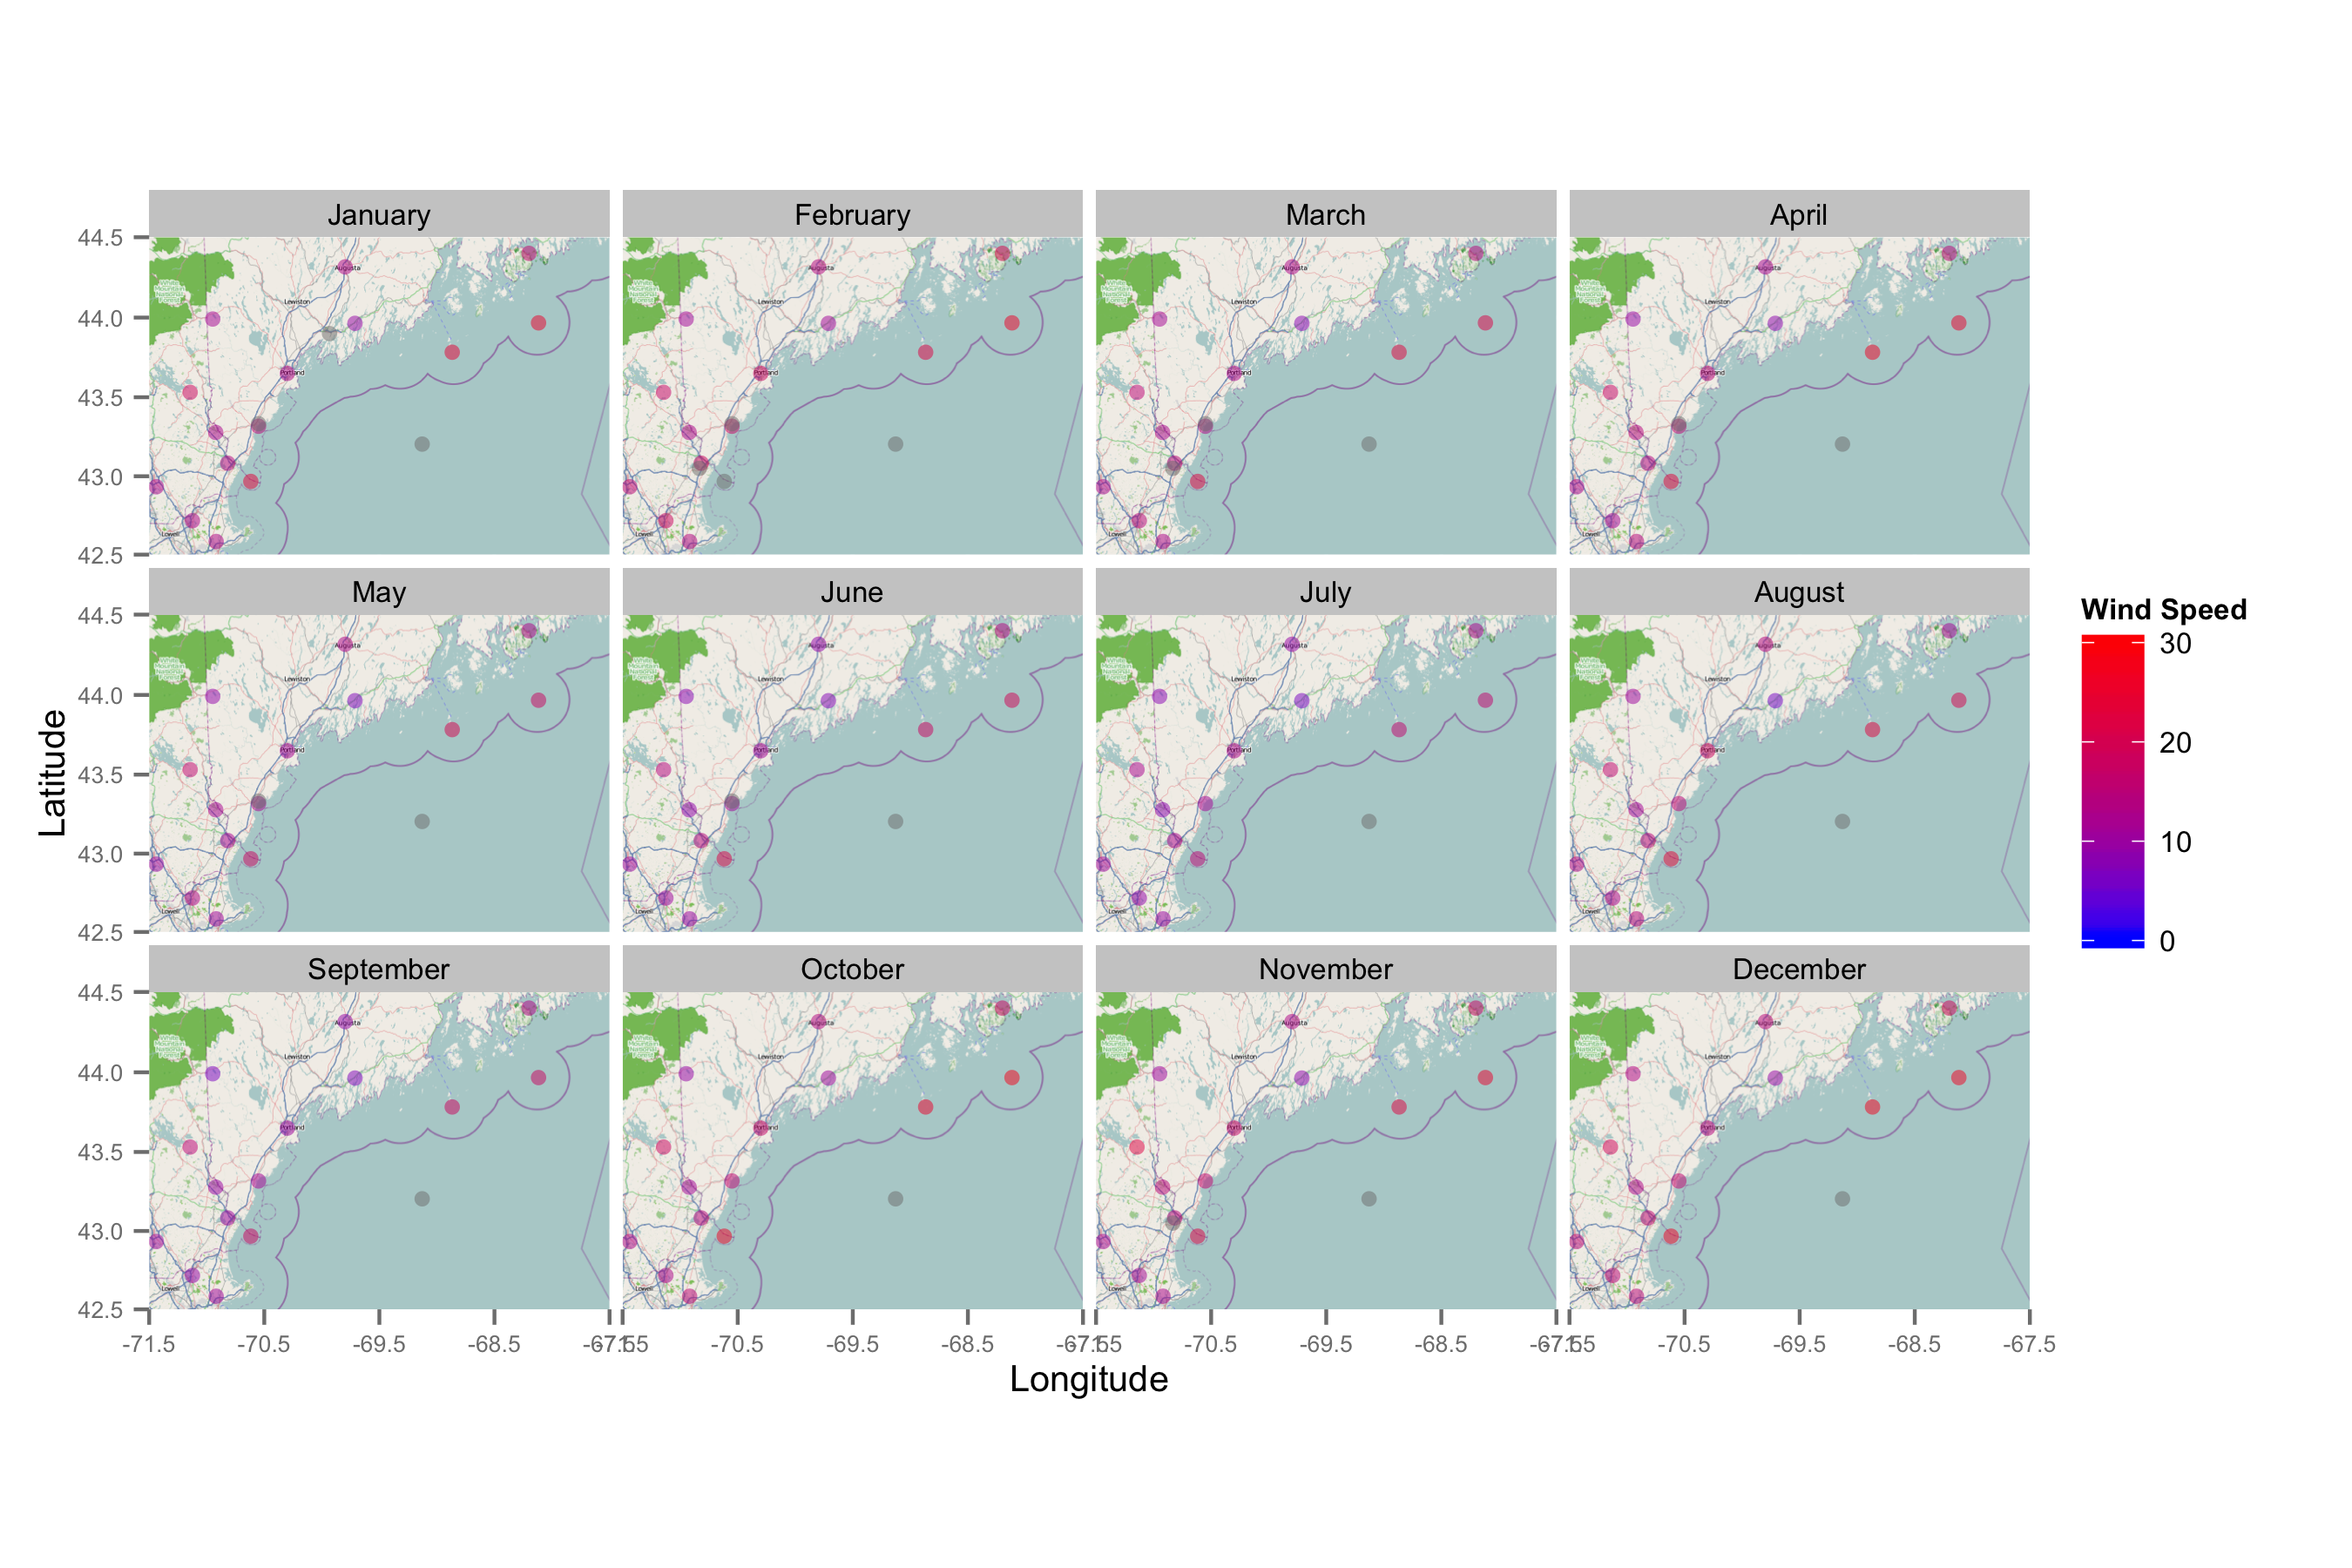
\includegraphics[width = 6in]{../maps/MapMonthlyMaximumWindSpeed}
\caption{Maximum wind speeds. Marker colors show the maximum of all measured wind speeds.}
\end{figure}

\chapter{Climatologies}
% wind speed
\begin{figure}[!ht]
\centering
\includegraphics[width = 6in]{../figures/PlotOfWindSpeedClimatology}
\caption{Wind speed climatologies. Plots show the maximum, mean daily maximum, mean daily mean, mean daily minimum and maximum wind speed each month for all of the stations in the study area.}
\end{figure}

% temperature
\begin{figure}[!ht]
\centering
\includegraphics[width = 6in]{../figures/PlotOfTemperatureClimatology}
\caption{Temperature climatologies. Plots show the maximum, mean daily maximum, mean daily mean, mean daily minimum and maximum temperature each month for all of the stations in the study area.}
\end{figure}


\appendix
\chapter{Station Climatologies}
\clearpage
\input{StationsList}

\end{document}  